% This must be in the first 5 lines to tell arXiv to use pdfLaTeX, which is strongly recommended.
\pdfoutput=1
\documentclass[11pt]{article}
\usepackage{acl}
\usepackage{times}
\usepackage{latexsym}
\usepackage{soul}
\usepackage{xcolor}
\usepackage{tikz}
\usepackage{pgfplots}
\pgfplotsset{compat=1.18} 
\usepackage[T1]{fontenc}
\usepackage[utf8]{inputenc}
\usepackage{microtype}
\usepackage{amsmath}
\usepackage{algorithm}
\usepackage[noend]{algpseudocode}

\title{Multilingual Emotion Recognition in Conversation}

\author{Junyin Chen {} {} {} Hanshu Ding {} {} {} Zoe Fang {} {} {} Yifan Jiang \\
		\texttt{\{junyinc, hsding99, zoekfang, yfjiang\}@uw.edu} \\
        Department of Linguistics \\ University of Washington}

\begin{document}
\maketitle
\begin{abstract}
  TBD
\end{abstract}

\section{Introduction}
TBD

\section{Task Description}

\subsection{Primary Task}
\label{sect:primary_task}

Our primary task is emotion recognition in conversation (ERC) task on the text modality of the Multimodal EmotionLines Dataset (MELD). The dataset is in English and contains dialogues and utterances from TV series scripts . We will predict the emotion for each utterance from dialogues involving multiple speakers.

\subsubsection{Dataset}

MELD\citep{poria-etal-2019-meld} \footnote{\url{https://affective-meld.github.io/}}, also kown as \textit{Multimodel Emotionlines Dataset}, is a multi-party emotional conversational database that is extended from Emotionlines dataset. 
Emotionlines \citep{hsu-etal-2018-emotionlines}\footnote{\url{http://doraemon.iis.sinica.edu.tw/emotionlines/index.html}} dataset is an emotion dialogue dataset with emotion labels for each utterance. The utterances are collected from Friends TV scripts and private Facebook messenger dialogues. Each utterance is labeled with one of Ekman’s six basic emotions plus the neutral emotion. MELD is an upgraded emotion dataset that contains about 13,000 utterances from 1,433 dialogues from only the TV-series Friends. Each utterance in MELD is annotated with emotion and sentiment labels, and encompasses audio, visual, and textual modalities. 
MELD split the dataset into training, development, and testing set separately (1039 dialogues for training set, 114 dialogues for developing set and 280 dialogues for testing set). We use the testing set and corresponding gold standard annotation for analysis.

According to Poria, the speakers of these dialogues were categorized to 6 main characters and others. The utterances are distributed relatively evenly with respect to speakers (from 12\% to 16\%).  The emotion distribution for each character is also similar. 


\subsection{Adaptation Task}
\label{sect:adaptation_task}

Our adaptation task is to adapt our model to Chinese dialogues in the Multi-party Dialogue Dataset (MPDD). Other dimensions for this task remain the same as the primary task.

\subsubsection{Dataset}

Multi-party Dialogue Dataset (MPDD) \citep{chen-etal-2020-mpdd} \footnote{\url{http://nlg.csie.ntu.edu.tw/nlpresource/MPDD}} is a Chinese emotional conversational dataset. The dataset contains a total of 25, 548 utterances from 4, 142 dialogues, which are collected from five TV series scripts from \url{www.juban108.com}. Each uttrance is annmotated with three types of labels: emotion, relation, and target listener. In particular, the emotion labels are consistent with those in the Emotionlines dataset.


\section{System Overview}
\label{sec:overview}

\subsection{Design}

Instead of appending the correspondent speaker tag with the utterance for training, we integrate the ideology of having a multi-task deep neural network that shares the lower layer across multiple single-sentence and pairwise text classification tasks. 

With the benefit of multi-task deep neural network, we enable our model to gain context awareness with multiple context related tags, such as speaker, past and future utterance.

\subsection{Methodology}

We want to determine the emotion of a specific utterance in a dialogue group $M$, which contains multiple speakers in speaker group $S$. The dialogue group $M$ can be expressed as a list of vectors: $dialogue = [x_1, x_2, ..., x_{n-1}, x_n]$, where each utterance contains multiple words. The correspondent speaker list can be expressed as another list of vectors: $speaker = [s_1, s_1, ..., s_2, s_3]$, where $s_n$ is in the speaker group $S$. Since this is a supervised setup, we will utilize the manually labeled emotion label $e_n$ corresponding to each utterance $x_n$ in the dialogue group $M$.

The simplest solution is to have a function $f$ that takes each utterance $x_t$ as input and output the correct label $e_t$. For our setup, we decide on a multi-tasking function $f$ to output correspondent speaker $s_t$, as we want to take the speaker into account. Furthermore, we add past utterance $[x_1, x_2, ..., x_{t-1}]$ and even future utterance $[x_{t+1}, x_{t+2}, ..., x_n]$, as we anticipate adding more context around the utterance for analysis will further improve the result.


\subsection{Algorithm}

For each task in the multi-task deep neural network, we use the pretrained "Roberta-base" model \citet{liu-etal-2019-multi}. We choose BERT like algorithms as they both have simple structure, and support more than one segment for tokenization. We choose to use RoBERTa as the main algorithm for training, facilitating result comparison with results listed in \citet{kim-2021-emoberta}. Even though pre-trained BERT and RoBERTa models do not expect more than two segments as inputs, both Kim et al. and us show that having more than two segments improves evaluation results.

We will have either two or three segments, if we want to include both past and future utterances.


\section{Approach}
\label{sec:approach}

\subsection{Problem Statement}
MELD provides information on the speaker and turn (in the dialogue) of each utterance. We want to take these two factors into account and build a model that learns speaker-specific features and the context of an utterance. At the same time, we want to build a multi-task model to accomplish both tasks at the same time.


\subsection{Model Architecture}

We build a Multi-Task Deep Neural Networks (MP-DNN) Model \citet{liu-etal-2019-multi} to train both Emotionlines and MPDD data so that the model can learn shared knowledge between two datasets. We use a pre-trained RoBERTa base encoder transformer for the initial text embeddings. On top of the shared pre-trained transformer encoder, we build two different task-specific models for each task. \\
To manipulate the inputs, we either add some context or provide the speaker information. The caveat of training a MP-DNN on top of RoBERTa is that the latter is previosuly trained with inputs no longer than two sentences, where each two sentence has a BOS \textit{<s>} token and an EOS \textit{</s>} token. When we concatenate more than one past utterance to the to-predict utterance, we strip the EOS token of the past utterances and keep only one that exists between the context and the to-predict utterance. Algorithm 1 shows our preprocessing algorithm of adding context information.
\begin{algorithm}
\caption{Add All Past Utterance(s)}\label{euclid}
\begin{algorithmic}[1]
\State \textbf{Given} an $Uttr$ and its $idx$ in dialogue
\If {$idx \neq 0$}
    \State $i \gets 1$
    \While {$idx - i \geq 0$}
        \State $Uttr_{past} \gets Data_{idx-i}$
        \State $Speaker_{past} \gets Uttr_{Past_{speaker}}$
        \State $str \gets Speaker_{past} + Uttr_{Past}$
        \State $Context \gets Context + str$
        \State $i \gets i + 1$
    \EndWhile
\EndIf
\State $Uttr_{curr} \gets Context + EOS + Uttr$
\end{algorithmic}
\end{algorithm}

\subsection{Evaluation}

Both tasks will be evaluated using weighted F1 to account for the imbalance of the dataset. We will also evaluate the error rate between predicted the true emotion labels that are labelled manually by the dataset curators. 


\section{Results}
\label{sec:results}

\begin{table}[hbt]
  \centering
  \begin{tabular}{c|c|c}
    past utterance & future utterance & weighted F1 \\
    \hline
    0 & 0 & 60.17 \\
    \hline
    0 & 6 & 61.96 \\
    \hline
    6 & 0 & 62.46 \\
    \hline
    6 & 6 & \hl{62.56} \\
  \end{tabular}
  \caption{Weighted F1 when number of past or future utterances are added as context.}
\end{table}

Using our evaluation metric, the model currently yields a 62.56 percent weighted F1 score. This accuracy fluctuates within a small range when we change the inputs to the model. That is, accuracy on test data can vary by in 1.2 percent when the model receives inputs with(out) speaker information or past/future utterances. Table 1 shows the result under different model setups

\begin{table}[hbt]
  \centering
  \begin{tabular}{c|c|c|c}
    emotion & true count & total count & accuracy \\
    \hline
    neutral & 1026 & 1256 & 81.69 \\
    \hline
    joy & 247 & 402 & 61.44 \\
    \hline
    anger & 156 & 281 & 55.52 \\
    \hline
    surprise & 173 & 345 & 50.14 \\
    \hline
    sadness & 66 & 208 & 31.73 \\
    \hline
    disgust & 5 & 68 & 7.35 \\
    \hline
    fear & 1 & 50 & 2.00 \\
  \end{tabular}
  \caption{Weighted F1 when number of past or future utterances are added as context.}
\end{table}

The prediction output and accuracy is shown as below in Table 2. It is obvious that the prediction for emotion 'neutral' is easier compared to other types. Also, it is interesting that the accuracy for the prediction of specific emotions decreases with the decreasing number of learning instances for the corresponding emotions. 

Besides, we also noticed that there was a high tendency for non-neutral emotions to be predicted as 'neutral' emotions (323 out of 936 misprediction). Oppositely, for real neutral emotions, they are likely to be predicted as 'joy' or 'surprise'.

\begin{figure}
\centering
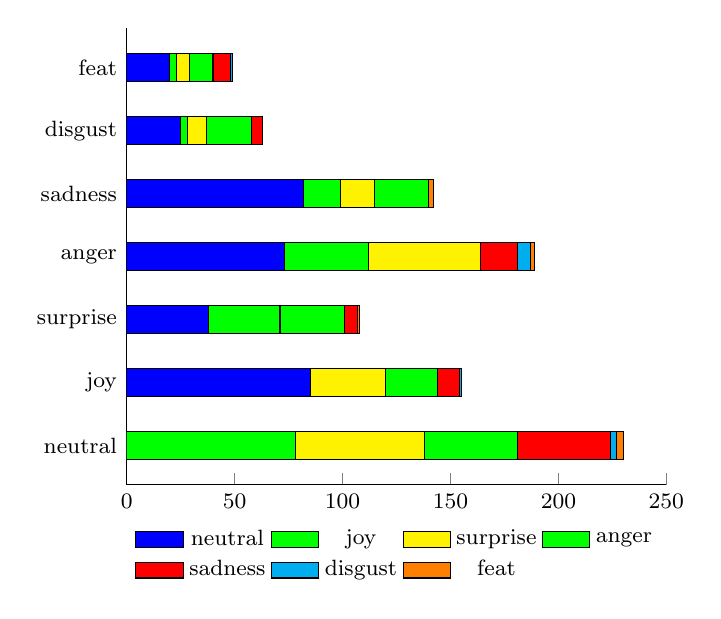
\begin{tikzpicture}
\begin{axis}[
    xbar stacked,
    legend style={
    legend columns=4,
        at={(xticklabel cs:0.5)},
        anchor=north,
        draw=none
    },
    ytick=data,
    axis y line*=none,
    axis x line*=bottom,
    tick label style={font=\footnotesize},
    legend style={font=\footnotesize},
    label style={font=\footnotesize},
    xtick={0,50,100,150,200,250},
    xlabel={Time in ms},
    yticklabels={neutral, joy, surprise, anger, sadness, disgust, feat},
    xmin=0,
    xmax=250,
    area legend,
    y=8mm,
    enlarge y limits={abs=0.625},
]
\addplot[fill=blue] coordinates
{(0,0) (85,1) (38,2) (73,3) (82,4) (25,5) (20, 6)};
\addplot[fill=green] coordinates
{(78,0) (0,1) (33,2) (39,3) (17,4) (3,5) (3, 6)};
\addplot[fill=yellow] coordinates
{(60,0) (35,1) (0,2) (52,3) (16,4) (9,5) (6, 6)};
\addplot[fill=green] coordinates
{(43,0) (24,1) (30,2) (0,3) (25,4) (21,5) (11, 6)};
\addplot[fill=red] coordinates
{(43,0) (10,1) (6,2) (17,3) (0,4) (5,5) (8, 6)};
\addplot[fill=cyan] coordinates
{(3,0) (1,1) (0,2) (6,3) (0,4) (0,5) (1, 6)};
\addplot[fill=orange] coordinates
{(3,0) (0,1) (1,2) (2,3) (2,4) (0,5) (0, 6)};
\legend{neutral, joy, surprise, anger, sadness, disgust, feat}
\end{axis}  
\end{tikzpicture}
\caption{The distribution of mis-predicted emotions}
\label{fig:stats}
\end{figure}

\section{Discussion}

\subsection{Pre-trained model decision}

Using RoBERTA-base pre-trained model, we achieve similar result illustrated in Kim et al. However, using RoBERTa-full pre-trained model used by Kim et al., weighted F1 score reduced by as much as 30 percent, regardless of number of past or future utterances included in the training dataset.

\subsection{Number of past and future utterance.}

Adding future utterance alone does not greatly improve the result. The result of adding future utterance alone is similar of having no future or past utterance. Adding both past and future utterance, preforms almost the same as adding only past utterance. 

\subsection{Qualitative Analysis}

We did a qualitative analysis with on 10 correctly and 10 incorrectly classified random sample from the test split. For all the incorrectly classified random sample, the speaker tags are all incorrectly classified. For the 10 correctly classified random sample, 40 percent of the speaker tags are correctly classified. This shows that having speaker tag does help improve the result, but not as substantial as we hopped. 

\begin{quote}

<s>\hl{Mon}ica:Is that too much to ask after six year\hl{?!}\hl{Mon}ica:I \hl{mean}, all I’m asking for is just a little emotio\hl{!} \hl{Ch}andler:And you’re upset because you didn’t make your \hl{best} friend cry?</s></s>I mean \hl{what}?</s>

\end{quote}

An incorrectly classified example. The prediction is surprise while the truth is anger. The predicted speaker is Rachel while the true speaker is Monica.

\begin{quote}

<s>\hl{Rachel}\hl{:}Oh, that sounds great.Others:\hl{How} does that \hl{sound}?Others:Well, I’ve got a project for you that’s a lot more related to fashion.Others\hl{:}Well, don’t think I haven’t noticed your potential.Rachel\hl{:}Oh, you got me.Others\hl{:}Eh.</s></s>Come on over here, sweetheart\hl{.}</s>

\end{quote}

A correctly classified example. Both the prediction and truth are neutral. Both the predicted speaker and the true speaker are Others. \\

We initially anticipate that the speaker tag will be utilized for sentiment classification. However, both the incorrectly and correctly classified example, the <s> token in the last layer mainly focus on punctuation marks. This phenomenon far deviates from Kim et al.'s result, that <s> token mainly focus on the speaker in correctly classified examples. This proves that separating speaker and utterance for speaker detection does not benefit the model to utilize speaker context for sentiment analysis.

Furthermore, the RoBERTa pre-trained tokenizer tokenized Mon from Monica and Ch from Chandler. We suspect incorrect tokenization of the Speaker may further deteriorate the result, as the model may not correctly utilize the speaker tags in past or future utterance for current utterance's sentiment analysis.


\section{Conclusion}
\label{sect:conclusion}

TBD

% Entries for the entire Anthology, followed by custom entries
\bibliography{anthology, custom}

\end{document}
